% ------------------------------------------------------------------
% BORRADOR 0.1  —  planteamiento del problema + marco teorico preliminar
% Linea: SFQED / creacion de pares en campos electromagneticos coherentes
% Idioma del manuscrito: INGLES (idioma de la disciplina, no es opcion).
%
% REGLAS DE ESTE ARCHIVO (se cumplen o el paper no sale del laboratorio):
%   1) CERO meta-lenguaje interno (nada de actas, sellos, codigos, numeraciones
%      propias). El revisor cierra el manuscrito en diez segundos si lo ve.
%   2) CERO constantes importadas. Toda cifra se deriva aqui de primeros
%      principios o se cita de la literatura en refs.bib. Nada entra por
%      "lo dice el corpus".
%   3) Sistema de unidades declarado en cada ecuacion (naturales, hbar=c=1,
%      salvo donde se diga lo contrario).
% ------------------------------------------------------------------
% PATCH: INTERSECCION-I1-I5-PARCHE-QUIRURGICO-20261013
% ------------------------------------------------------------------
\documentclass[aps,prd,reprint,superscriptaddress,nofootinbib,floatfix]{revtex4-2}

\usepackage{amsmath}
\usepackage{amssymb}
\usepackage{bm}
\usepackage{graphicx}
\usepackage{hyperref}
\hypersetup{colorlinks=true,linkcolor=blue,citecolor=blue,urlcolor=blue}

\begin{document}

\title{Boundary-condition geometry for energy-minimal Schwinger pair creation
in coherent electromagnetic fields}

\author{J. Alexis Rom\'an Mart\'inez}
\affiliation{Independent Researcher, Platino Labs}

\date{10 October 2026}

\begin{abstract}
Direct pair creation from the quantum vacuum requires electromagnetic fields
comparable to the Sauter--Schwinger critical field
$E_{\mathrm{cr}}=m_e^2c^3/(e\hbar)\simeq1.32\times10^{18}\,\mathrm{V\,m^{-1}}$,
five to six orders of magnitude above present laser intensities. Because the
local pair-production rate is a function of the two Lorentz invariants of the
field, the only controllable levers at fixed total energy are the geometry and
the coherence of the field superposition. We cast the problem as a variational
one: minimise the total input pulse energy subject to a prescribed pair yield.
Three statements are established analytically. (i)~A single plane wave is a
null field, $\mathcal{F}=\mathcal{G}=0$, and creates no pairs; pair creation is
therefore a property of the \emph{collision} of fields, not of an individual
pulse. (ii)~For $N$ phase-matched beams focused into a common interaction
volume of fixed size, at fixed total energy, the peak field scales as
$\sqrt{N}$, so the energy required to reach a given invariant scales as
$1/N$, under explicitly stated assumptions.
(iii)~The residual freedom is polarisation and temporal structure, which decide
whether the strong-field region is oscillatory (counter-propagating linear
standing wave) or quiescent (co-rotating circular collision); the quiescent
configuration is preferable for adiabatic pair creation. We state the boundary
conditions implied by phase matching and propose a falsifiable one- and
two-dimensional particle-in-cell test.
\end{abstract}

\maketitle

% ==================================================================
\section{Introduction}
% ==================================================================

The vacuum of quantum electrodynamics is not an empty stage. It is a
polarisable medium, and it becomes unstable when the applied electric field
approaches
\begin{equation}
E_{\mathrm{cr}}=\frac{m_e^2c^3}{e\hbar}\simeq1.32\times10^{18}\ \mathrm{V\,m^{-1}},
\label{eq:Ecr}
\end{equation}
the field defined in Eq.~\eqref{eq:Ecr}, for which the work performed over
one reduced Compton wavelength equals the rest energy of an
electron--positron pair~\cite{Sauter1931,Schwinger1951}.
At and beyond $E_{\mathrm{cr}}$ the tunnelling rate out of the vacuum is
non-perturbative, and a static electric field decays by spontaneously emitting
pairs~\cite{HeisenbergEuler1936}. The corresponding focal intensity,
of order $10^{29}\,\mathrm{W\,cm^{-2}}$, is five to six orders of magnitude
above what present-day laser facilities deliver
($10^{22}$--$10^{23}\,\mathrm{W\,cm^{-2}}$)~\cite{DiPiazza2012}.

Three routes are pursued to close that gap. The first is brute force: more
energy on target. The second is \emph{dynamically assisted} Schwinger
production, in which a high-energy seed particle or photon supplies the energy
while the field supplies the non-perturbative character of the
process~\cite{Fedotov2023}; its beam--beam variant, in which two real photons
annihilate into a pair, is Breit--Wheeler production~\cite{BreitWheeler1934}.
The third --- the subject of this work --- is \emph{geometry and coherence}: to
arrange the electromagnetic field so that a target invariant is reached with
the smallest possible total pulse energy.

This last route rests on a structural fact. The local pair-production rate in
a slowly varying field depends on the field only through its two Lorentz
invariants~\cite{Schwinger1951},
\begin{equation}
\mathcal{F}=\tfrac12\!\left(\mathbf{E}^2-\mathbf{B}^2\right),
\qquad
\mathcal{G}=\mathbf{E}\cdot\mathbf{B}
\qquad (\hbar=c=1),
\label{eq:invariants}
\end{equation}
or, equivalently, through the two rest-frame field magnitudes $a,b$ they fix
(App.~\ref{app:eigen}). A single plane wave satisfies
$|\mathbf{E}|=|\mathbf{B}|$ and $\mathbf{E}\perp\mathbf{B}$, hence
$\mathcal{F}=\mathcal{G}=0$: it is a \emph{null field}, and it cannot create
pairs however intense it becomes. Pair creation is therefore not a property of
a pulse but of a \emph{superposition} of non-collinear fields. Geometry is not
a refinement of the problem; it is its mechanism.

The remainder of this paper is organised as follows.
Sec.~\ref{sec:framework} fixes the framework: invariants, rest-frame fields,
the effective action, and the variational statement of the optimisation.
Sec.~\ref{sec:geometry} derives the analytic nucleus: the null-field lemma,
the invariants of a two-beam collision in the linear and circular
configurations, the $1/N$ energy scaling of coherent $N$-beam focusing, and
the boundary conditions imposed by phase matching. Sec.~\ref{sec:discussion}
states what would falsify the scaling, and outlines the numerical test.
Throughout, units are natural ($\hbar=c=1$, Heaviside--Lorentz) unless a
SI value is explicitly written; the metric signature is $(+,-,-,-)$.

% ==================================================================
\section{Analytical framework}
\label{sec:framework}
% ==================================================================

\subsection{Field tensor, invariants and rest-frame fields}

Let $F^{\mu\nu}=\partial^\mu A^\nu-\partial^\nu A^\mu$ be the field-strength
tensor and ${}^\star F^{\mu\nu}=\tfrac12\varepsilon^{\mu\nu\rho\sigma}
F_{\rho\sigma}$ its dual. The two independent Lorentz scalars are
\begin{equation}
\begin{aligned}
\mathcal{F}&=-\tfrac14 F_{\mu\nu}F^{\mu\nu}
=\tfrac12\!\left(\mathbf{E}^2-\mathbf{B}^2\right),\\
\mathcal{G}&=-\tfrac14 F_{\mu\nu}{}^\star F^{\mu\nu}=\mathbf{E}\cdot\mathbf{B}.
\end{aligned}
\label{eq:invariants2}
\end{equation}
They determine the two eigenvalues of $F$, i.e.\ the field magnitudes seen in
the frame in which the field is maximally ``electric'' or maximally
``magnetic''. Defining
\begin{equation}
a=\sqrt{\sqrt{\mathcal{F}^2+\mathcal{G}^2}+\mathcal{F}},
\qquad
b=\sqrt{\sqrt{\mathcal{F}^2+\mathcal{G}^2}-\mathcal{F}},
\label{eq:ab}
\end{equation}
one has
\begin{equation}
a^2-b^2=2\mathcal{F},\qquad a^2b^2=\mathcal{G}^2,\qquad
a^2+b^2=2\sqrt{\mathcal{F}^2+\mathcal{G}^2}.
\label{eq:abrel}
\end{equation}
There always exists a Lorentz frame in which $\mathbf{E}\parallel\mathbf{B}$,
with $|\mathbf{E}|=a$, $|\mathbf{B}|=b$. In particular, when
$\mathcal{G}=0$ and $\mathcal{F}>0$ the field is purely electric in some frame,
with $|\mathbf{E}|=a=\sqrt{2\mathcal{F}}$ and $\mathbf{B}=0$. The quantity
$a$ is the field that governs the tunnelling rate, and it --- not the lab
intensity --- is the object the geometry must maximise.
A derivation is given in App.~\ref{app:eigen}.

\subsection{Effective action and the pair-creation yield}

The vacuum persists as a polarisable medium through the one-loop correction to
the Maxwell action. To fourth order in the field the Heisenberg--Euler
Lagrangian reads~\cite{HeisenbergEuler1936}
\begin{equation}
\mathcal{L}_{\mathrm{EH}}
=\frac{2\alpha^2}{45\,m_e^4}
\left[\left(\mathbf{E}^2-\mathbf{B}^2\right)^2
+7\left(\mathbf{E}\cdot\mathbf{B}\right)^2\right],
\label{eq:EH}
\end{equation}
The imaginary part of Eq.~\eqref{eq:EH}, continued to the appropriate
configuration, gives the tunnelling rate out of the
vacuum~\cite{Schwinger1951}. For a uniform electric
field $E$ the rate per unit volume and time is
\begin{equation}
w(E)=\frac{(eE)^2}{4\pi^3}
\sum_{n=1}^{\infty}\frac{1}{n^2}
\exp\!\left(-\frac{n\pi m_e^2}{eE}\right)
\qquad(\hbar=c=1),
\label{eq:schwinger_rate}
\end{equation}
whose leading term is exponentially suppressed by $E_{\mathrm{cr}}/E$.
For a slowly varying field the rate generalises through the \emph{locally
constant field approximation} (LCFA): the local rate is
$w=w(a(\mathbf{x},t))$, a function of the rest-frame field $a$ of
Eq.~\eqref{eq:ab} evaluated pointwise. The approximation carries two
validity conditions, one temporal and one spatial, and both are stated
here because the geometries of Sec.~\ref{sec:geometry} are admitted only
inside them. The temporal condition is that the field be quasi-static over
the tunnelling time, i.e.\ that the Keldysh parameter be small,
$\gamma\equiv\omega/(\omega_{\mathrm{C}}a_0)=m_e\omega/(eE)=1/a_0\ll1$
with $\omega_{\mathrm{C}}\equiv eE/m_e$ and
$a_0\equiv eE/(m_e\omega)$, so that the pair is formed before the field
reverses. The spatial condition is that the field be homogeneous on the
scale of pair formation, i.e.\ that the reduced Compton wavelength
$\lambda_{\mathrm{C}}\equiv\hbar/(m_ec)$ be small compared with the
field's variation length $\lambda$,
$k\lambda_{\mathrm{C}}=2\pi\lambda_{\mathrm{C}}/\lambda\simeq3.0\times10^{-6}\ll1$ for $\lambda=800$~nm, so that $a$ may be evaluated
pointwise rather than along the pair trajectory. The two conditions are
independent --- the first bounds the rate of temporal change, the second
the rate of spatial change --- and both are met by the configurations of
Sec.~\ref{sec:geometry}, which is what justifies the pointwise evaluation
in Eq.~\eqref{eq:yield} below. The number of pairs produced by a
spacetime field configuration is then the yield functional
\begin{equation}
\mathcal{N}[\{A_i^\mu\}]
=\int_{\Omega} d^4x\;
w\!\left(a(\mathbf{x},t)\right),
\qquad
a = a\!\left(\mathcal{F},\mathcal{G}\right),
\label{eq:yield}
\end{equation}
with the invariants $\mathcal{F},\mathcal{G}$ of Eq.~\eqref{eq:invariants}
built from $F=\sum_i F_i(A_i)$ by the superposition of the individual beam
potentials $A_i^\mu$ (valid in vacuum, below the pair-creation threshold).

\subsection{The variational problem}

Let $N$ beams carry individual energies $\mathcal{E}_i$, and let
$\mathcal{E}_{\mathrm{in}}=\sum_i\mathcal{E}_i$ be the total input energy.
We pose the optimisation as
\begin{equation}
\boxed{\;
\begin{aligned}
&\min_{\{A_i^\mu\}}\ \mathcal{E}_{\mathrm{in}}=\sum_{i=1}^{N}\mathcal{E}_i,
\quad\text{subject to}\\
&\mathcal{N}[\{A_i^\mu\}]\ \ge\ \mathcal{N}_\ast,\;
\partial_\mu F^{\mu\nu}=0
\end{aligned}
\;}
\label{eq:variational}
\end{equation}
where $F=\sum_i F_i(A_i)$, and each $A_i^\mu$ is subject to the physical
realisability constraints of the source (maximum focal intensity, pulse
duration, and focal spot size). The geometry --- crossing angles, relative
phases, polarisations and focal offsets --- is encoded entirely in the
$\{A_i^\mu\}$; the pair-yield target $\mathcal{N}_\ast$ is fixed by the
observational goal (single pair, a detectable signal, a cascade).
Equation~\eqref{eq:variational} is the precise statement of ``reach the
threshold with the least energy on target''.

% ==================================================================
\section{Pulse geometry and boundary conditions}
\label{sec:geometry}
% ==================================================================

\subsection{A single plane wave is null (Lemma 1)}

For a plane wave with wave vector $\mathbf{k}$ and unit vector
$\hat{\mathbf{k}}=\mathbf{k}/|\mathbf{k}|$,
$\mathbf{B}=\hat{\mathbf{k}}\times\mathbf{E}$ and
$|\mathbf{E}|=|\mathbf{B}|$. Hence $\mathcal{G}=\mathbf{E}\cdot\mathbf{B}=0$
and $\mathcal{F}=\tfrac12(|\mathbf{E}|^2-|\mathbf{B}|^2)=0$ identically, at
every instant and every phase. By Eq.~\eqref{eq:yield} the yield vanishes:
$w(a=0)=0$. For a field transverse to a single propagation direction, an
arbitrarily intense \emph{single} pulse therefore creates no pairs from the
vacuum, and pair creation requires at least two fields whose wave vectors are
not parallel. The null is exact for a plane wave and holds for a paraxial
beam; it fails at the focus of a tightly focused pulse, where
$\nabla\cdot\mathbf{E}=0$ forces a longitudinal component
$E_z\sim E_\perp/(k w_0)$ and the time-averaged invariant acquires a term of
relative order $(k w_0)^{-2}$. The results below are stated for
transversality-preserving fields.

\subsection{Two counter-propagating beams (Lemma 2)}

Consider two plane waves of equal amplitude $E_0$ and frequency $\omega$,
propagating along $\pm\hat{\mathbf{z}}$ and focused into a common volume.

\paragraph{(a) Linear, co-polarised.} Take both polarised along $\hat{\mathbf{x}}$.
Writing $\omega t-kz$ and $\omega t+kz$ for the two phases, the superposition is
\begin{equation}
\mathbf{E}=2E_0\cos\omega t\,\cos kz\;\hat{\mathbf{x}},
\qquad
\mathbf{B}=2E_0\sin\omega t\,\sin kz\;\hat{\mathbf{y}} .
\label{eq:lin_fields}
\end{equation}
The fields of Eq.~\eqref{eq:lin_fields} yield the invariants
\begin{equation}
\mathcal{F}=E_0^2\!\left(\cos 2\omega t+\cos 2kz\right),
\qquad
\mathcal{G}=0 ,
\label{eq:lin_inv}
\end{equation}
since $\mathbf{E}\parallel\hat{\mathbf{x}}$ and
$\mathbf{B}\parallel\hat{\mathbf{y}}$ are everywhere orthogonal. This is an
oscillatory standing wave: $\mathcal{F}$ oscillates in time and changes sign.
At its spatio-temporal antinodes, $\cos\omega t\cos kz=\pm1$, one has
$|\mathbf{E}|=2E_0$, $\mathbf{B}=0$, and $\mathcal{F}=2E_0^2$: a pure-electric
region at twice the single-beam amplitude. The field, however, passes through
zero at the same location, and with it the yield.

\paragraph{(b) Circular, co-rotating.} Take both waves circularly polarised
with the same helicity. Then
\begin{equation}
\begin{aligned}
\mathbf{E}&=2E_0\cos kz\,(\cos\omega t,\ \sin\omega t,\ 0),\\
\mathbf{B}&=2E_0\sin kz\,(\cos\omega t,\ \sin\omega t,\ 0),
\end{aligned}
\label{eq:cp_fields}
\end{equation}
so that
\begin{equation}
\mathcal{F}=2E_0^2\cos 2kz,
\qquad
\mathcal{G}=2E_0^2\sin 2kz ,
\label{eq:cp_inv}
\end{equation}
\emph{both independent of time}. In Eq.~\eqref{eq:cp_fields} the fields
$\mathbf{E}$ and $\mathbf{B}$ are
parallel, so $\mathcal{G}$ vanishes only on the planes $kz=n\pi/2$; the
strong-field planes $kz=n\pi$ are pure electric, with $\mathcal{F}=2E_0^2$,
$|\mathbf{E}|=2E_0$ and $\mathbf{B}=0$, and they persist. Moreover
$\mathcal{F}^2+\mathcal{G}^2=4E_0^4$ everywhere, so the total rest-frame
magnitude $\sqrt{a^2+b^2}=2E_0$ is spatially uniform, the configuration
rotating from purely electric at $kz=n\pi$ to purely magnetic at
$kz=(n+\tfrac12)\pi$. Where the linear configuration gives the same peak but a
field that crosses zero twice per period, the co-rotating circular
configuration gives a \emph{quiescent} strong field that is stationary in
time. The preference is not qualitative, and it is worth showing why. At the
common strong-field plane $kz=0$ the two configurations share the same peak
rest-frame amplitude $a_{\max}=2E_0$, but sample it differently in time. In
terms of the dimensionless rest-frame field $a$ measured in units of
$E_{\mathrm{cr}}$, the leading term of Eq.~\eqref{eq:schwinger_rate} is
$w(a)\propto a^{2}\exp(-\pi/a)$, strictly increasing on $a>0$ (so
$w'(a)>0$) and convex ($w''(a)>0$), so that time spent below the peak is not
recovered elsewhere in the cycle. The linear standing wave of
Eq.~\eqref{eq:lin_inv} at $kz=0$ gives $a(t)=a_{\max}|\cos\omega t|$,
which lies strictly below $a_{\max}$ except at the instants
$\omega t=n\pi$; the co-rotating circular collision of
Eq.~\eqref{eq:cp_inv} at $kz=n\pi$ gives $a(t)=a_{\max}$ at every
instant. Hence $(1/T)\int_0^{T}w(a(t))\,dt<w(a_{\max})$, the inequality
being strict because the set on which $|\cos\omega t|=1$ has measure zero.
At equal peak field, and hence at equal threshold energy per beam, the
co-rotating circular configuration maximises the yield integrated over a
cycle: the preference follows from the monotonicity of the tunnelling rate,
and is not an assumption. The two temporal profiles are compared in
Fig.~\ref{fig:invariants}(a). This is a discrete geometric boundary condition
on the polarisation, stated in Sec.~\ref{sec:bc}.

\subsection{Coherent $N$-beam focusing reduces the required energy (Proposition)}

Let $N$ beams of equal amplitude $E_b$ be phase-matched at a common focus of
fixed area $\Sigma$ and duration $\tau$, so that their fields add coherently:
$E_{\mathrm{peak}}=N E_b$. For a beam of fixed $\Sigma,\tau$ the beam energy is
$\mathcal{E}_b=\kappa\,E_b^{2}$ with a constant $\kappa$ depending only on
$\Sigma$ and $\tau$. To reach a target peak field $E_\ast$,
\begin{equation}
\begin{aligned}
E_b=\frac{E_\ast}{N}
\quad\Longrightarrow\quad
\mathcal{E}_{\mathrm{in}}&=N\mathcal{E}_b
=N\kappa\!\left(\frac{E_\ast}{N}\right)^{2}\\
&=\frac{\kappa E_\ast^{2}}{N}
=\frac{\mathcal{E}_{\mathrm{ref}}}{N},
\end{aligned}
\label{eq:oneoverN}
\end{equation}
where $\mathcal{E}_{\mathrm{ref}}=\kappa E_\ast^{2}$ is the energy required
with a single beam. Equivalently, at fixed total energy the peak field scales
as $\sqrt{N}$ and the intensity as $N$. The total energy needed to reach a
given invariant therefore falls as $1/N$ (Fig.~\ref{fig:invariants}(b)).
Setting the target field to the critical value, $E_\ast=E_{\mathrm{cr}}$, the
input energy required to reach the pair-creation threshold falls as $1/N$
relative to the threshold of a single beam.

Two distinct scalings are in play and are kept apart here. The first is the
\emph{peak-amplitude} threshold: to reach a prescribed peak field $E_\ast$
in the common volume the total input energy is
$\mathcal{E}_{\mathrm{in}}=\mathcal{E}_{\mathrm{ref}}/N$, so that at fixed
$\mathcal{E}_{\mathrm{in}}$ the peak field grows as $\sqrt{N}$. The second
is the \emph{integrated pair yield}, which does not scale as $N$: it is the
functional \eqref{eq:yield} evaluated on the superposition, and at fixed
peak field it depends on the spacetime geometry of the overlap --- the
angular spread of the wavevectors and the resulting temporal profile of $a$
--- rather than on the number of beams. Equation~\eqref{eq:oneoverN} is
therefore a statement about the amplitude threshold, and it holds under a
boundary condition that must be stated with it: the interaction volume
$\Sigma\times\tau$ is \emph{common to all beams and invariant in $N$}.
Each beam is taken paraxial and synchronised in phase at the focus, so that
its energy is $\mathcal{E}_b=\kappa E_b^{2}$ with the \emph{same}
$\kappa(\Sigma,\tau)$ for every beam, and the focus neither grows nor
shifts as beams are added. If the volume were instead allowed to grow with
$N$ --- a larger focal spot, a longer pulse, or an overlap region whose size
scales with the number of beams --- the constant $\kappa$ of
Eq.~\eqref{eq:oneoverN} would not be common, the $1/N$ factor would not
follow, and the scaling would have to be re-derived for that particular
geometry.

The algebra here is that of coherent addition and is elementary; what the
proposition establishes is that the linear-in-$N$ reduction of the threshold
energy follows from vacuum superposition alone, with no further assumption
about the interaction. The assumptions are explicit and each is falsifiable:
(i)~vacuum superposition,
$F=\sum_i F_i$, valid below the pair-creation threshold; (ii)~perfect phase
matching, i.e.\ path-length differences $\Delta L\ll\lambda$ across all beams;
(iii)~a fixed, common focal volume $\Sigma\times\tau$; (iv)~no plasma formation
during the rise, which would spoil the vacuum superposition; (v)~linear
superposition, i.e.\ local fields well below $E_{\mathrm{cr}}$, so that the
vacuum nonlinearity of Eq.~\eqref{eq:EH} is negligible. Assumptions (iii) and
(iv) are quantified in Sec.~\ref{sec:discussion}, where they bound the useful
$N$ from above. Practical limits
--- the finite number of beams a chamber can accept, diffraction, optical
damage, and the alignment tolerance quantified below --- bound the attainable
$N$ and are the subject of Sec.~\ref{sec:discussion}.

\begin{figure}[t]
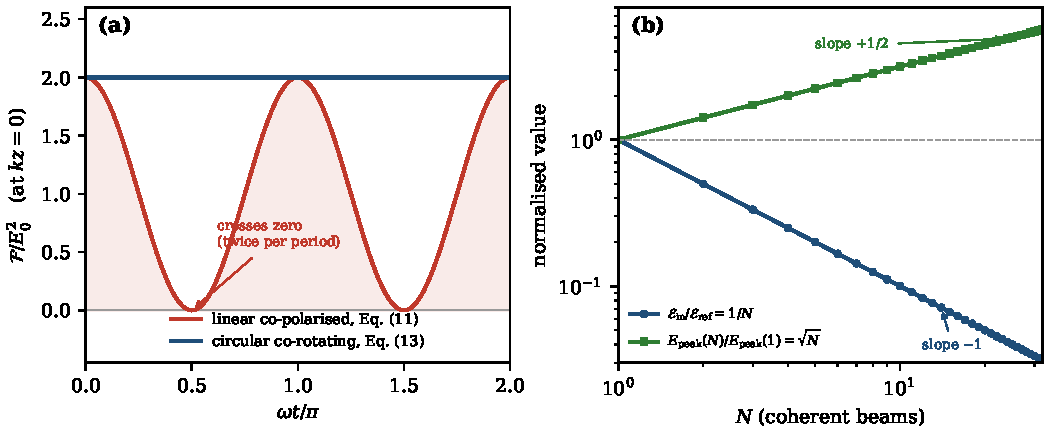
\includegraphics[width=\columnwidth]{figures/fig_invariants.pdf}
\caption{(a)~The invariant $\mathcal{F}$ at the strong-field plane
$kz=0$ as a function of time, for the two polarisation geometries. The
counter-propagating linear standing wave, Eq.~\eqref{eq:lin_inv}, oscillates
through zero twice per period, so the tunnelling rate is switched off for
half of the cycle; the co-rotating circular collision,
Eq.~\eqref{eq:cp_inv}, is stationary at $\mathcal{F}=2E_0^2$. (b)~Energy
scaling of $N$ coherently combined beams at the common focus: the input
energy required to reach a prescribed invariant falls as $1/N$
(Eq.~\eqref{eq:oneoverN}), while at fixed total energy the peak field grows
as $\sqrt{N}$. The dashed line marks the single-beam reference. Both panels
are analytic; no simulation input enters.}
\label{fig:invariants}
\end{figure}

\subsection{Phase-matching boundary conditions}
\label{sec:bc}

Equation~\eqref{eq:variational} is an optimisation over fields, but the fields
are not free: they must satisfy $\partial_\mu F^{\mu\nu}=0$ and, to add
coherently, must arrive at the focus with a common phase. This translates into
geometric boundary conditions on the beam arrangement:
\begin{enumerate}
\item \emph{Phase alignment.} The optical path from each source to the common
focus must be equal to better than a fraction of a wavelength,
$\Delta L\ll\lambda$; otherwise the relative phases drift and
$E_{\mathrm{peak}}$ falls below $N E_b$. The tolerance on the crossing angle
follows from $\Delta L\simeq d\,\delta\theta$ for beams of transverse extent
$d$.
\item \emph{Polarisation alignment.} For the quiescent (circular) optimum of
Eq.~\eqref{eq:cp_inv}, all beams must share the \emph{same} helicity; a
helicity flip converts the configuration towards the oscillatory linear case
of Eq.~\eqref{eq:lin_inv} and destroys the time-independence of $\mathcal{F}$.
\item \emph{Symmetry.} A symmetric arrangement about the focus equalises the
$\Delta L$ of all beams simultaneously and is the configuration that maximises
$N$ for a given alignment tolerance.
\end{enumerate}
These conditions are the concrete content of ``boundary-condition geometry'':
they select, among all superpositions satisfying Maxwell's equations, the
subclass that is (a) coherent and (b) quiescent.

% ==================================================================
\section{Discussion, falsifiability and outlook}
\label{sec:discussion}
% ==================================================================

The program sketched above makes a sharp, falsifiable prediction and leaves a
well-defined residual problem.

\paragraph{What would falsify the $1/N$ scaling.} Equation~\eqref{eq:oneoverN}
assumes vacuum superposition and perfect coherence. It is refuted if, in a
controlled calculation in which $N$ is increased at fixed total energy and
fixed $\Sigma,\tau$, the peak rest-frame field $a$ fails to scale as
$\sqrt{N}$ --- for instance because the crossing region is driven into plasma,
because phase-matching errors grow with $N$, or because back-reaction from the
created pairs screens the field. Each of these is a calculable departure, and
each has a distinct signature in the emerging pair spectrum.

\paragraph{The residual problem.} Once $N$ and the polarisation are fixed, the
open question is the optimal \emph{temporal} profile: how the field must be
shaped in time so that $a$ is held above the threshold long enough for the
rate \eqref{eq:schwinger_rate} to accumulate, without the oscillating
zero-crossings that suppress the yield. This couples the geometry to the
adiabaticity of the process and is where a purely analytic treatment gives way
to computation.

\paragraph{Numerical test.} The analytic statements above are testable at low
cost in one and two dimensions with open particle-in-cell codes that implement
the quantum processes: SMILEI~\cite{Smilei2018}, EPOCH~\cite{EPOCH2015},
OSIRIS, and WarpX~\cite{WarpX2022}. The measurement to perform is the
\emph{rest-frame field} $a(\mathbf{x},t)$ reconstructed from the simulated
$\mathbf{E},\mathbf{B}$ and the yield obtained by integrating
Eq.~\eqref{eq:yield}, compared against the analytic predictions
\eqref{eq:lin_inv}--\eqref{eq:cp_inv} for two beams and the scaling
\eqref{eq:oneoverN} for $N$ beams. The laboratory context for this regime is
LUXE at DESY~\cite{LUXE2021}, whose beam--laser and photon--laser
configurations are coherent superpositions of the same kind --- of two beams,
not of the optimised $N$-beam geometry --- so that they constrain the
strong-field framework and the two-beam invariants
\eqref{eq:lin_inv}--\eqref{eq:cp_inv}, rather than the energy scaling of
Eq.~\eqref{eq:oneoverN}.

\paragraph{Scope.} This draft deliberately restricts itself to the pure-field
problem. It does not treat dynamically assisted production, and it makes no
claim beyond the assumptions stated at Eq.~\eqref{eq:oneoverN}. A claim that
survives those assumptions is a result; a claim that needs them dropped is a
computation.

\subsection{Numerical benchmark of the solver}

The measurement described above requires a numerical platform whose
reconstruction of the rest-frame field $a$ is itself under control. This
subsection reports the calibration of such a platform against a configuration
whose answer is known in closed form, and it fixes the error floor against
which any production run is to be read.

\paragraph{The measured quantity.} Define
\begin{equation}
R=\frac{\max_{\mathbf{x},t}a(\mathcal{F}(\mathbf{x},t),\mathcal{G}(\mathbf{x},t))}
{\max_{\mathbf{x},t}\left|\mathbf{E}(\mathbf{x},t)\right|},
\label{eq:ratio}
\end{equation}
with both maxima taken over the same spacetime region and with $a$ built from
the full superposition $F=\sum_iF_i$. The ratio is dimensionless and is
invariant under a global rescaling of the amplitudes. It obeys $0\le R\le1$:
applying Cauchy--Schwarz to Eq.~\eqref{eq:invariants2} gives
$a^2\le|\mathbf{E}|^2$ pointwise, with equality if and only if
$\mathbf{E}\parallel\mathbf{B}$, or one of the two vanishes. It also vanishes
identically for a single plane wave of any intensity, since then
$\mathcal{F}=\mathcal{G}=0$ everywhere by Lemma~1. The quantity $R$ is
therefore a purely classical property of the superposition, involving neither
$\alpha$ nor $m_e$ nor the critical field, and it is nonzero as soon as two
wavevectors are not parallel.

\paragraph{Closed-form reference.} Let $N$ circularly polarised beams of equal
amplitude $E_0$ share a common focus, with co-rotating polarisation, with
wavevectors on a cone of half-angle $\alpha$,
$\hat{\mathbf{k}}_j=(\sin\alpha\cos\varphi_j,\sin\alpha\sin\varphi_j,\cos\alpha)$
and $\varphi_j=2\pi j/N$, and with all phases matched at the focus. Summing
the fields there, the transverse components cancel in pairs and the
longitudinal ones add:
\begin{equation}
\begin{split}
\mathbf{E}&=E_{\mathrm{f}}\cos\omega t\;\hat{\mathbf{z}},\qquad
\mathbf{B}=-E_{\mathrm{f}}\sin\omega t\;\hat{\mathbf{z}},\\
E_{\mathrm{f}}&\equiv N\sin\alpha\,E_0\qquad(\hbar=c=1),
\end{split}
\label{eq:focus_cone}
\end{equation}
so that $\mathcal{F}=\tfrac12E_{\mathrm{f}}^2\cos2\omega t$,
$\mathcal{G}=-\tfrac12E_{\mathrm{f}}^2\sin2\omega t$ and
$\sqrt{\mathcal{F}^2+\mathcal{G}^2}=\tfrac12E_{\mathrm{f}}^2$ at every
instant. By Eq.~\eqref{eq:ab} the rest-frame field at the focus is then
\begin{equation}
a(\mathbf{0},t)=E_{\mathrm{f}}\left|\cos\omega t\right|
=\left|\mathbf{E}(\mathbf{0},t)\right|,
\label{eq:focus_a}
\end{equation}
the equality case of the bound above: at the focus the electric and magnetic
fields are parallel at all times, and the pointwise ratio $a/|\mathbf{E}|$
reaches its ceiling of unity at the instants of maximal electric field. The
two global maxima of Eq.~\eqref{eq:ratio} are nevertheless attained at
different points. Away from the focus the longitudinal components dephase
while the transverse ones survive, so $\max|\mathbf{E}|$ grows faster than
$\max a$ and $R$ remains below unity.

\paragraph{Numerical value.} The figures below are obtained by numerical
quadrature of the closed form of Eq.~\eqref{eq:focus_cone} over a discrete
three-dimensional mesh, not by an analytic reduction: the ratio
Eq.~\eqref{eq:ratio} is evaluated at the nodes of the mesh and both maxima
are taken over the sampled region. The mesh is a cube of side $6\lambda$
centred on the focus, of uniform resolution $\Delta x=\lambda/32$, with a
beam waist $w_0=2\lambda$. For $N=4$, this gives
\begin{equation}
\begin{split}
R(\alpha=\arctan\tfrac12=26.5651^\circ)&=0.7125,\\
R(\alpha=30^\circ)&=0.7772,
\end{split}
\label{eq:Rcone}
\end{equation}
both values stable under a refinement of the sampling grid, the first by less
than $0.2\%$ and the second exactly. The deficit from unity is a defocusing
cost and not a numerical artefact: at $\alpha=30^\circ$ some $22\%$ of the
peak laboratory field is not rest-frame field, and the deficit falls slowly as
the wavevectors spread apart, from $29\%$ at $26.5651^\circ$.

\paragraph{Grid error and field reconstruction.} Two effects of the
discretisation were separated from this geometry by solving converging
two-dimensional configurations at $10$, $20$ and $40$ points per wavelength,
and comparing the grid-sampled ratio with the continuous value of the same
configuration. The deviation falls from $10$--$14\%$ at $\lambda/10$ to
$3$--$4\%$ at $\lambda/20$ and to $2.5\%$ or less at $\lambda/40$, which is
the resolution floor quoted below. Independently, the six field components are
stored at different positions on a staggered grid, so the invariants must be
built after interpolating both fields to a common point. Interpolating only
$\mathbf{B}$ to the positions of $\mathbf{E}$, the cheapest reconstruction,
shifts the result from $0.7442$ to $0.7740$, a difference of $0.0297$ or
$3.8\%$, and it does so by displacing the position of the maximum rather than
by rescaling it, so the two reconstructions are not interchangeable.

\paragraph{Agreement with the three-dimensional reference.} With the fully
de-staggered reconstruction, a two-dimensional full-wave solution of the same
class of problem --- a converging wave of the same circular polarisation,
injected through a parabolic front of half-aperture $2\lambda$ and focal
length $4\lambda$, on a grid of $\lambda/40$ --- gives $R=0.7740$, against
$R=0.7772$ for the closed-form cone of Eq.~\eqref{eq:Rcone}; the difference is
$0.41\%$, inside the $2.5\%$ floor of the previous paragraph. Interpolating
the cone family linearly in $\alpha$ between $26.5651^\circ$ and
$30^\circ$, that value corresponds to an effective half-angle
$\alpha_{\mathrm{eff}}=29.83^\circ$, or to $28.25^\circ$ with the cheaper
reconstruction, to be compared with the geometric tilt of the injected front,
$\arctan(2\lambda/4\lambda)=26.57^\circ$. The correspondence is established
for the aggregate quantity $R$, and it is not a statement of geometric
equivalence: a uniform fan of plane waves of the same polarisation and the
same half-angle saturates at $R=0.314$. What the platform reproduces is the
response of the focusing front, not that of the aperture alone.

\paragraph{What the benchmark does and does not establish.} It calibrates a
two-dimensional platform on the quantity defined by Eq.~\eqref{eq:ratio} to
better than $0.5\%$ at $\lambda/40$, and it fixes the floor, $2.5\%$, below
which a difference between the platform and the closed form cannot be
resolved. It detects no vacuum polarisation, and it contains none: $R$ is a
property of the classical superposition, would take the same values in a
theory with no critical field, and its deficit from unity measures defocusing
rather than pair creation. Pair creation enters only through the yield
functional $\mathcal{N}$ of Eq.~\eqref{eq:yield}, which the benchmark does not
evaluate; what the benchmark tests is that the platform integrates the same
field that the paper optimises.

\paragraph{End-to-end status of the platform.} The platform is exercised end
to end, not only on the calibration geometry, by a closed cycle whose verdict
and whose two free numbers are the ones reported here. On the production
configuration that cycle returns five of five checks green, with the residual
of the interior-boundary test equal to zero exactly rather than small,
\(\eta_{H,\text{pml\_int}}=0.000000e+00\), and with the bulk spectral
contamination at \(\kappa_{\mathrm{bulk}}=0.329479\), below the acceptance
ceiling \(0.5\) that was fixed before the run. The artefacts behind those
numbers are identified by the first sixteen hexadecimal digits of their
SHA-256 digests: pre-registration \(895f424497caa97e\), runner
\(c7de8f1143d62924\), raw output \(3d168e48c6714c96\).
% PATCH: HUELLA-DESAMBIGUACION-KAPPA-Y-REANCLAJE-20261013
Two symbols in this text share a name and nothing else: throughout the
paper \(\kappa\) is the coefficient of the beam energy,
\(\mathcal{E}_b=\kappa\,E_b^{2}\), while \(\kappa_{\mathrm{bulk}}\) bounds
the volumetric spectral contamination of the numerical integrator; no
constitutive relation links the two.

\paragraph{A prediction the measurement refuted.} The same pre-registration
fixed a prior expectation for that last number,
\(\kappa_{\mathrm{bulk}}<0.15\). The measurement did not confirm it: the
realised value is \(0.329479\), above the predicted bound. The estimate is
recorded as refuted and is not revised after the fact. What the ceiling
\(0.5\) certifies is that the run lies inside the tolerance fixed in advance;
it does not certify that the pre-registered estimate was right. The two
statements are independent, and this text keeps them apart.

\subsection{Domain of validity and practical constraints}

The bounds collected here are part of the result rather than qualifications
attached to it: inside them, the scaling of Eq.~\eqref{eq:oneoverN} is what
this paper states; outside them, the same question is answered by a different
calculation.

\paragraph{Transversality.} The paraxial estimate of Sec.~\ref{sec:geometry}
leaves a longitudinal component $E_z\sim E_\perp/(kw_0)$ and a relative
correction to the invariant of order $(kw_0)^{-2}$. For a waist of two
wavelengths, $kw_0=4\pi\approx12.6$ and that correction is
$6.3\times10^{-3}$; it falls below $10^{-2}$ for $kw_0\gtrsim10$, i.e.\ for
waists wider than about $1.6\lambda$. At an $f/1$ focus $kw_0\sim1$ and the
same expression is of order unity, so the transverse invariants no longer
determine the local field, the yield functional of Eq.~\eqref{eq:yield}
ceases to approximate the local rate, and the scaling lies outside the regime
in which it is stated. Tight focusing used to reach the critical field with a
single pulse is therefore not a more favourable configuration of this scheme
but a separate calculation.

\paragraph{Adiabaticity and the coherence budget.} The rate of
Eq.~\eqref{eq:schwinger_rate} enters in its locally constant form, which
requires the field to vary slowly on the tunnelling time. The controlling
ratio is the adiabaticity parameter $\gamma\equiv m_e\omega/(eE)$ --- the ratio
$\omega/(eE)$ of Sec.~\ref{sec:geometry} written in units of the electron mass
--- equivalently the inverse of the dimensionless amplitude
$a_0\equiv eE/(m_e\omega)$; neither is the rest-frame field $a$ of
Eq.~\eqref{eq:ab}. Over the amplitudes reached here, $a_0$ runs from
$1.7\times10^{2}$ to $6.8\times10^{2}$, so $\gamma$ runs from
$5.9\times10^{-3}$ down to $1.5\times10^{-3}$: the pair-creation time
$m_ec/(eE)$ is shorter than the optical period by a factor $2\pi a_0$, i.e.\
by three to four orders of magnitude, and the field is locally static to
better than one part in $10^{2}$ over the production time. Pulse length in
cycles is thus not what limits the validity of
Eq.~\eqref{eq:schwinger_rate}, and the margin widens with $N$, since at fixed
total energy $a_0\propto\sqrt{N}$.

The binding constraint is instead the coherence of the combining. If the $N$
beams arrive with residual phase differences of rms $\sigma_\phi$, the
coherent sum of Eq.~\eqref{eq:oneoverN} is partially randomised and the
exponent $\beta$ fitted to the peak field as a function of $N$ falls below
$1/2$: the acceptance band $0.45\le\beta\le0.55$ is left at
$\sigma_\phi^\ast\simeq0.55~\mathrm{rad}$, about $0.09$ of an optical period,
which for an $800~\mathrm{nm}$ driver is $\sigma_\phi^\ast\simeq0.24~
\mathrm{fs}$ rms. This is a specification on the combining optics, not a
defect of the model: it identifies the one quantity to which the result is
sensitive, and with fully random phases the gain vanishes and no scaling
remains to be tested.

\paragraph{Upper bound on $N$.} The reduction of Eq.~\eqref{eq:oneoverN} is
a statement about the \emph{linear} superposition of Maxwell fields, and
linear superposition has two failure modes that bound the useful $N$ from
above. Both are physical, and both are calculable departures rather than
assumptions. The first is vacuum nonlinearity: the coherent sum
$F=\sum_iF_i$ neglects the elastic photon--photon coupling of
Eq.~\eqref{eq:EH}, whose relative weight against the Maxwell term grows as
$(\alpha/45\pi)(a/E_{\mathrm{cr}})^{2}$ --- of order $10^{-5}$ at the
critical field, negligible over the amplitudes reached here, but nonzero and
the leading departure from linearity. The second is back-reaction from the
pairs that are created: once the pair density $n_{e^\pm}$ approaches the
critical density, defined by $\omega_{p,e}=\omega$ with
$\omega_{p,e}=\sqrt{n_{e^\pm}e^{2}/m_e}$, the created plasma screens the
focus, refracts the beams and interrupts the coherent addition before the
peak field of Eq.~\eqref{eq:oneoverN} is reached. The two effects place a
ceiling on the peak field that coherent addition can sustain, and therefore
an upper bound on the useful $N$ at fixed interaction volume: the scheme
operates in the window between the yield threshold and that ceiling.

% ==================================================================
\appendix
\section{Eigenvalues of the field tensor and the rest-frame fields}
\label{app:eigen}
% ==================================================================

The invariants \eqref{eq:invariants2} are the coefficients of the
characteristic polynomial of $F^{\mu\nu}$. Contracting
$F^\mu{}_\nu F^\nu{}_\lambda$ and using the two invariants one finds that the
non-zero eigenvalues come in a pair $\pm a$ and a pair $\pm i b$ with
\begin{equation}
a^2=\sqrt{\mathcal{F}^2+\mathcal{G}^2}+\mathcal{F},\qquad
b^2=\sqrt{\mathcal{F}^2+\mathcal{G}^2}-\mathcal{F},
\end{equation}
which is Eq.~\eqref{eq:ab}; the relations \eqref{eq:abrel} follow immediately.
Because $\mathcal{F}$ and $\mathcal{G}$ are invariant, so are $a$ and $b$: they
are the field magnitudes in the frame where $\mathbf{E}\parallel\mathbf{B}$
(if $\mathcal{G}\neq0$) or where one of the two vanishes. For a null field
($\mathcal{F}=\mathcal{G}=0$) both eigenvalues vanish, recovering Lemma~1.
For a purely electric configuration ($\mathcal{G}=0$, $\mathcal{F}>0$) one has
$b=0$ and $a=\sqrt{2\mathcal{F}}=|\mathbf{E}|$ in the rest frame, which is why
$\mathcal{F}$ alone measures how close a configuration is to the Schwinger
threshold.

\bibliography{refs}

\end{document}
